\chapter{Программная реализация}

\section{Модель}
\section{Обучение}
\section{Предсказание}

\subsection{Постобработка}
Сырой выход модели представляет из себя тензор таких же размеров, что и вход,
содержащий для каждой точки входа вероятность наличия активации в ней. Однако
нас интересуют конкретные активации.

\section{Подсчет метрик}

После получения предсказания встает вопрос о подсчете метрик, ведь при прямом
сравнении, метки с предсказания и с разметки могут быть смещены относительно
друг друга, например, на несколько сэмплов. С учетом пожеланий предметного
специалиста, для исследований которого предоставлялось разметка, было решено
считать истинно положительной активацию, которая была предсказана с точностью
до 5 сэмплов.

Таким образом алгоритм подсчета выглядел следующим образом:

Для подсчета TP и FP производилась итерация по активациям предсказания. В
окрестности в 5 сэмплов от каждой метки производился поиск наличия таковой в
исходной разметке. В случае положительного результата предсказание считалось
как TP, иначе --- FP. Для подсчета FN итерация происходила по активациям исходной
разметке, а поиск --- по предсказанию. Активация считалась FN в случае
отсутствия результатов поиска в окрестности истинной метки. Наглядно это
изображено на рис. \ref{fig:metrics} (желтым выделен сигнал, по меткам которого
происходит итерация).

\begin{figure}[!htb]
	\centering
	\subfigure[]{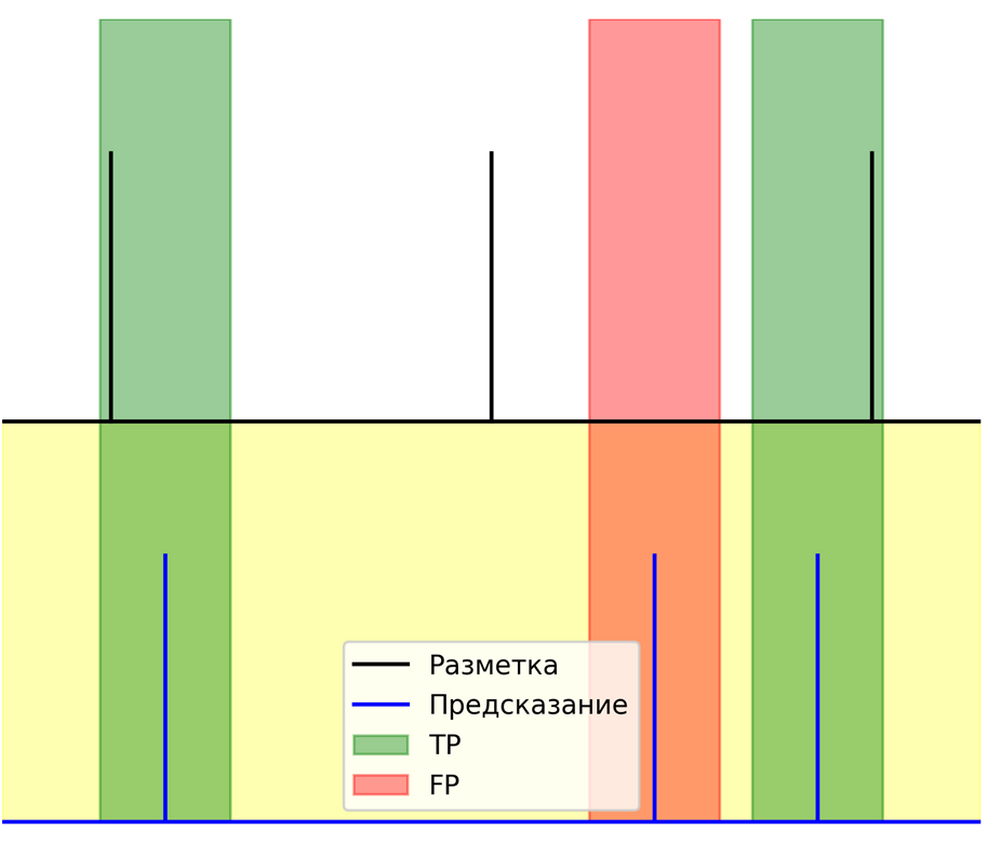
\includegraphics[width=.49\textwidth]{metrics1.png}}
	\subfigure[]{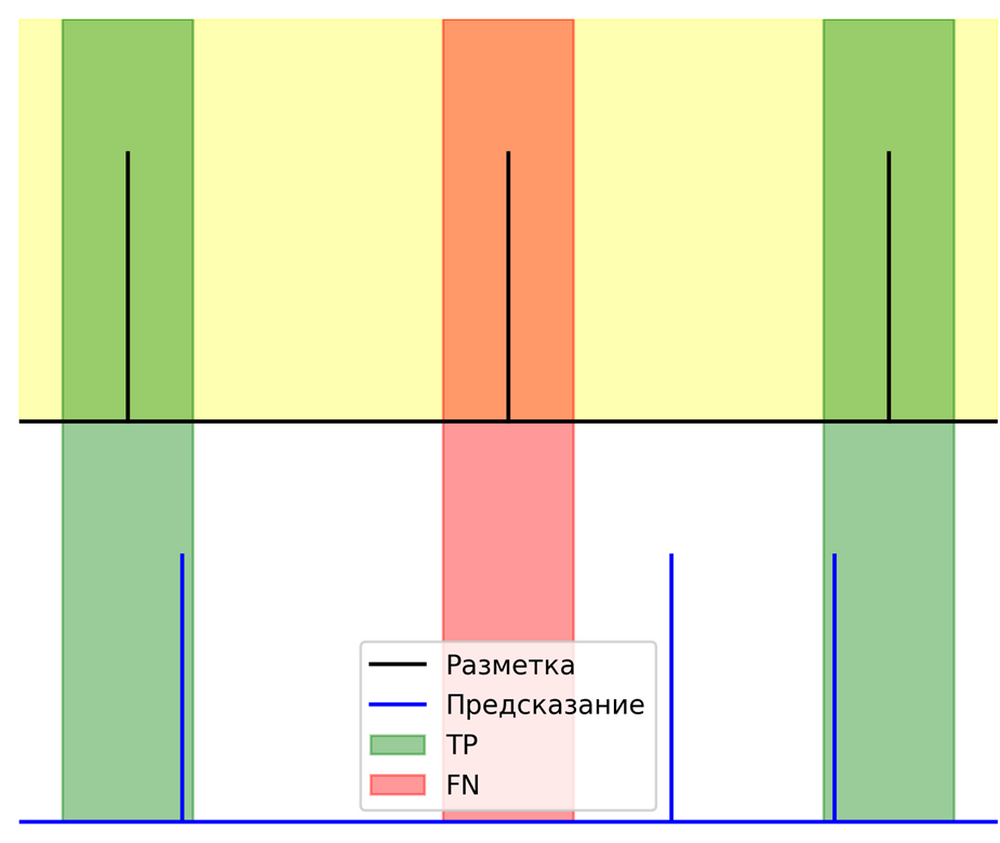
\includegraphics[width=.49\textwidth]{metrics2.png}}
	\caption{(a) Подсчет TP и FP (b) Подсчет FN}
	\label{fig:metrics}
\end{figure}

После подсчета TP, FP и FN по формулам, описанным выше, вычисляется $F_1score$.
